\chapter{Technologien für Multi-Wan Bonding}
\label{chap:verwendeteTechnologien}
\section{IP Routing Table}
Der IP Routing Table oder Routing Table ist eine Tabelle, die alle Hosts, die an einem Netzwerk angeschlossen sind, aufbauen. Diese Tabelle wird von dem Betriebssystem verwendet um IP Pakete weiter- oder umzuleiten. Durch diese Informationen ist es außerdem möglich die Topologie des Netzwerkes, in dem sich der Host befindet, zu bestimmen.\footnote[1]{\cite[Vgl.][]{2}}
\\\\
Einträge in das Routing Table können entweder manuell, in Form von statischen Routen oder dynamisch, über Routing Protokolle erstellt werden.$^{1}$
\\\\
Ein Eintrag des Routing Table unter Linux und unter Windows hat folgende 5 Attribute: ein Netzwerkziel, eine Netzwerkmaske, ein Gateway, eine Schnittstelle und eine Metrik.$^{1}$
\\\\
Das Netzwerkziel und die Netzwerkmaske zusammen beschreiben, an welches Netzwerk ein IP Paket gerichtet sein muss, um von diesem Eintrag beeinflusst zu werden. Hier gibt es jedoch eine besondere Einstellung, wenn das Netzwerkziel als auch die Netzwerkmaske nur aus Nullen besteht. Diese Einträge werden als default Routen bezeichnet. Default Routen beeinflussen alle Pakete, bei denen folgendes \textbf{nicht} zutrifft$^{1}$: 
\\
\begin{itemize}
    \item Es gibt keinen anderen default Routen mit einer niedrigeren Metrik.
    \item Pakete wurden vorher noch nicht von einem spezifischeren Eintrag umgeleitet.
\end{itemize}
\ \\
Das Gateway beschreibt den nächsten Hop. Genauer gesagt spiegelt es die IP-Adresse des Hosts wieder, um welches das IP-Paket umgeleitet werden muss, um in das Zielnetzwerk, oder in ein Netzwerk, das mit dem Zielnetzwerk verbunden ist, zu gelangen.$^{1}$
\\\\
Die Metrik gibt an, welcher Eintrag verwendet werden soll, wenn mehrere Einträge gleiche Werte im Netzwerkziel und in der Netzwerkmaske haben. Sie gibt bei dynamischen Routen an, wie viele Hops das IP Paket braucht, um beim Gateway anzukommen. Deswegen wird auch die kleinere Metrik bevorzugt, weil weniger Hops in der Regel weniger Latenz bedeuteten.$^{1}$
\newpage
\noindent
Die Schnittstelle gibt an, über welche Network Interface Card (NIC) das IP Paket geleitet werden muss, damit es das Gateway erreichen kann.\footnote[1]{\cite[Vgl.][]{2}}
\\\\
Eine Routing Tabelle kann wie folgt aussehen:
\\
\begin{center}
    \begin{tabular}{| c | c | c | c | c |}
        \hline
        Netzwerkziel & Netzwerkmaske & Gateway & Schnittstelle & Metrik \\
        \hline
        0.0.0.0 & 0.0.0.0 & 172.168.0.10 & 172.168.0.1 & 30 \\
        172.163.241.22 & 255.255.255.255 & 10.0.0.2 & 10.0.0.1 & 22 \\
        \hline
    \end{tabular}
\end{center}
\ \\
Bei diesem Beispiel wird ein Paket mit der IP-Adresse 172.163.241.22 an die IP-Adresse 10.0.0.2 über die Schnittstelle 10.0.0.1 weitergeleitet. Ein Paket mit IP-Adresse 30.20.10.0 wird an die IP-Adresse 172.168.0.10 über die Schnittstelle 172.168.0.1 weitergeleitet.


\section{Virtuelles privates Netzwerk}
Ein Virtuelles privates Netzwerk kurz VPN verwendet das Internet, um Daten verschlüsselt zu übertragen. Dies wird gemacht, indem die VPN Software die Daten beim Nutzer verschlüsselt und der Server sie wieder entschlüsselt. Die Vertraulichkeit, Integrität und Authentizität der Daten wird mithilfe von Verschlüsselungstechniken gewährt. Hier hat sich Internet Protocol Security (IPsec)\footnote[1]{\cite[Vgl.][]{31}} als Standard etabliert.\footnote[2]{\cite[Vgl.][]{29}}
\\\\
VPN wird von Firmen und auch von Privatpersonen genutzt. Firmen verwenden VPN, um ihren Mitarbeitern die Möglichkeit zu geben, von außerhalb des Firmennetzwerkes auf die Daten und Geräte der Firma zuzugreifen. Die private Nutzung von VPNs besteht darin, dass Nutzer Geoblocking umgehen wollen oder ihren Netzwerkverkehr sicherer gestalten wollen. Um Geoblocking zu umgehen werden Server von den VPN Anbietern auf der ganzen Welt verfügbar gemacht. Die Nutzer verbinden sich zu einem Server, senden die Anfrage, die Sie eigentlich an eine URL senden würden an diesen. Der Server sendet die Anfrage dann an die URL und schickt die Antwort zurück zu dem Nutzer, somit wirkt es für den Webserver so als würde der Nutzer aus dem Land kommen, wo der Server steht.$^{2}$
\begin{figure}[H]
    \centering
    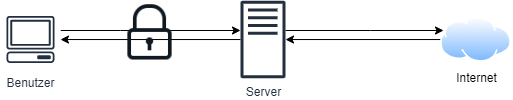
\includegraphics[width=0.8\textwidth]{VPN.png}
    \caption[VPN]{VPN} 
\end{figure} 

\newpage
\section{Interprozesskommunikation}
Interprozesskommunikation ist der Fachbegriff für die Kommunikation zwischen verschiedenen Prozessen auf demselben Rechner. Es gibt verschiedene Arten der Interprozesskommunikation, zum einen speicherbasierte Kommunikation in Form von Shared Memory oder Dateinen und zum anderen nachrichtenbasierte Kommunikation über Message Queues, Pipes oder Sockets.\footnote[1]{\cite[Vgl.][]{30}} 


\subsection{Shared Memory}
Mehrere Prozesse greifen auf gemeinsam genutzten Speicher lesend oder schreibend zu. Der Speicher wird von einem Prozess angefordert und dann mithilfe des Betriebssystems auch in den Adressraum der anderen Prozesse eingefügt, sodass jeder Prozess darauf zugreifen kann. Shared Memory ist eine sehr simple Form der Interprozesskommunikation, die einzige Schwierigkeit ist die Synchronisation der Prozesse, also das kein Prozess gleichzeitig mit einem anderen Prozess auf den gemeinsam genutzten Speicher zugreifen kann und es somit zu keinen Race Conditions kommt.$^{1}$


\subsection{Dateien}
Mehrere Prozesse greifen auf eine Datei zu, in diese Datei werden Daten von den Prozessen geschrieben beziehungsweise gelesen. Die Prozesse dürfen wie auch auf den Shared Memory nur synchronisiert zugreifen, oftmals erfolgt dies mithilfe des Betriebssystems das den Zugriff entweder auf nur einzelne Daten der Datei oder auf die ganze Datei sperrt.$^{1}$

\subsection{Message Queue}
Daten werden an eine Nachrichtenwarteschlange gesendet, diese hat eine eindeutige Kennung, sodass die anderen Prozesse wissen aus welcher Warteschlange sie die Daten beziehen müssen. Message Queues arbeiten entweder nach dem FIFO-Prinzip (First in First out) also die Daten, die als Erstes in die Warteschlange kommen, gehen auch als Erstes wieder raus oder mithilfe von Prioritäten, sodass Prozesse die Daten mit der höchsten Priorität als Erstes aus der Warteschlange nehmen.$^{1}$ 

\subsection{Pipes}
Die Pipe ist die erste Technik der Interprozesskommunikation, sie wurde für Unix entwickelt. Pipes kann man immer nur in eine Richtung verwenden, also ein Prozess schreibt immer und einer liest immer.  Um also Daten von einem Prozess zum anderen und wieder zurückzubefördern werden zwei unterschiedliche Pipes benötigt. Pipes sind wie auch die Massage Queues nach dem FIFO Prinzip aufgebaut. Es gibt zwei verschiedene Arten von Pipes die normalen/namenlosen Pipes und die benannten/FIFO Pipes. Der wesentliche Unterschied ist das namenlose Pipes nur von verwandten Prozessen verwendet werden können. Hingegen zu benannten Pipes die von jedem Prozess verwendet werden können, der den Namen der Pipe und die benötigten Berechtigungen hat, um eine Verbindung mit der Pipe aufzubauen.$^{1}$

\subsection{Sockets}
Zur Kommunikation mithilfe von Sockets wird ein Server und mindestens ein Client benötigt. Der Server hat  zu jedem Client ein Socket worüber er mit diesem kommunizieren kann. Die Kommunikation erfolgt in beide Richtungen. Der Plan für Sockets war das damit verschiedene Rechner über das Netzwerk miteinander kommunizieren können. Es ist aber auch möglich damit Interprozesskommunikation zu betreiben. Indem der Server und der Client beide am selben Rechner laufen.\footnote[1]{\cite[Vgl.][]{30}}